\chapter{Results}

\section{Mouse tissue development as a model system to study mRNA and tRNA gene
regulation}

Organogenesis during mouse development is a well-understood process (McLin and
Zorn 2006; Bruneau 2008; Zorn and Wells 2009; Si-Tayeb et al. 2010; Kang et al.
2011). For example, the molecular landscape within the liver is known to undergo
radical changes during development in response to shifts in the liver’s
physiological functions during embryogenesis.. During early development, the
embryonic liver is a haematopoetic organ; at birth, the neonatal liver becomes
the pri\-ma\-ry metabolic and detoxification organ (Si-Tayeb et al. 2010); at
weaning, further metabolic pathways are upregulated (Bohme et al. 1983; Girard
et al. 1992). In the developing brain, coordinated gene expression changes in a
heterogeneous collection of diverse cell types shape the functional
specialization of specific regions in both embryonic and postnatal brains
(Liscovitch and Chechik 2013; Sunkin et al. 2013).

To characterize changes in the mRNA and tRNA transcriptomes during
development,\todo{Make it sound sexy}
we performed strand-specific, total RNA-seq, as well as ChIP-seq against Pol~III
in C57BL/6J mice in liver and brain at the following developmental stages: two
embryonic (E15.5 and E18.5), two post-birth (P0.5 and P4) and immediately pre-
and post-weaning (P22 and P29) stages (Fig.~\ref{fig:design}). For each
experiment at each tissue and developmental stage, we performed two biological
replicates that were highly correlated (Methods, Supplemental Fig.~1–3). This
approach allowed us to quantify expression levels for protein-coding genes, as
well as Pol~III occupancy at every tRNA locus, which quantitatively captures the
utilization of each tRNA gene (Barski et al. 2010; Moqtaderi et al. 2010; Oler
et al. 2010; Kutter et al. 2011; Canella et al. 2012; Carriere et al. 2012;
Renaud et al. 2014).

\begin{figure}
    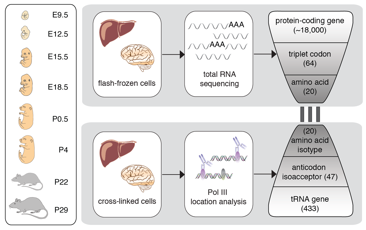
\includegraphics{experimental-design}

    \caption{\captitle{Transcriptome-wide analysis of protein-coding and tRNA
        genes during mouse organ development.}
        Liver and brain tissues were isolated at eight mouse developmental
        stages. Tissue samples were flash-frozen for RNA-sequencing (RNA-seq)
        and cross-linked using formaldehyde to preserve protein–DNA interactions
        for ChIP-sequencing (ChIP-seq) of Pol~III. Using the RNA-seq data we
        calculated from all expressed protein-coding genes the frequencies of
        each triplet codon for all 64 possible codons and 20 amino acids.
        Similarly, Pol~III binding to tRNA genes in the mouse genome was
        collapsed into 47 anticodon isoacceptor families and 20 amino acid
        isotypes (Methods). The bars linking RNA- and ChIP-seq data represent
        the three-nucleotide interactions between codon and anticodon. Pol~III
        occupancy was determined also in E9.5 (whole embryo) and E12.5 (head
        versus remaining body).\label{fig:design}}
\end{figure}

\section{Dynamic changes in protein-coding gene expression during mouse
development}

\todo{explain this section properly}

As expected, between stages we saw large-scale changes in the expression of
protein-coding genes known to have different functions during liver and brain
development (Li et al. 2009; Kang et al. 2011; Lee et al. 2012; Liscovitch and
Chechik 2013). For instance, \gene{ApoB}, which is the primary apolipoprotein
carrying low-density lipoproteins, is steadily upregulated during development;
in contrast, α-fetoprotein (\gene{Afp}), the fetal version of serum albumin, is
the primary circulatory carrier protein that over development is downregulated
and replaced by its adult counterpart (Chen et al. 1997; Lee et al. 2012)
(Fig.~2A, Supplemental Table 1). By performing matched RNA-seq experiments
during brain development, we observed similar dynamics of gene expression
rewiring at the neural transcription factor \gene{Foxp2}, where transcription
decreases steadily after birth, and at the neurotransmitter calmodulin
(\gene{Calm1}), where transcription increases after birth (Huang et al. 2011;
Tsui et al. 2013) (Fig.~2B, Supplemental Table 2).
